\chapter*{Введение}

В настоящее время как в нашей стране, так и за рубежом всё большее внимание уделяется созданию различных типов бепсилотных летательных аппаратов. В конструктировании таких самолетов особое внимание уделяется требованиям малозаметности и увеличения аэродинамического качества, и как следствие, возможности барражировать в течение длительного времени. 

Это связано с тем обстоятельством, что беспилотные летательные аппараты имеют ряд преимуществ перед пилотируемыми, в частности для них:
\begin{enumerate}
\item существенно менее жесткие требования по безопасности конструкции
\item не требуется систем поддержания работоспособности и жизнеобеспечения экипажа
\item существенно менее жесткие ограничения режимов полета.
\end{enumerate} 

Благодаря этому БПЛА имеют большой потенциал для разработки для них легких и дешевых конструкций планера, что позволяет решать многие технические задачи, недоступные для пилотируемых летательных аппаратов.

Рассказать про беспилотник (типы, картинки), предназначены для решения ряда задач.

Дальше про разные типы.

Основное - мониторинг (военный, гражданский). Из этого следуют требования малозаметности и весовой эффективности.

Использование беспилотника может обеспечить преимущество по сравнению с пилотируемыми, почему.

Показать несколько существующих и разрабатываемых БПЛА для мониторинга.

Конструкция этих планеров представляет собой интегральную схему с крылом большого удлинения, что зачастую приводит к выбору схемы летающего крыла.

Объясняем, почему нужна интегральная схема и крыло большого удлинения. Цель - меньше заметности следовательно уменьшение строительной высоты, больше аэродинамического качество.

Выходим на основную проблему. Проблема интеграции двигателя и центроплана. Описанные выше требования приводят к проблемам. 

Показываем наш БПЛА (модель из катьи), одним из решений является изогнутый центроплан.

\begin{figure}[ht]
\captionsetup{justification=centering}
\centering
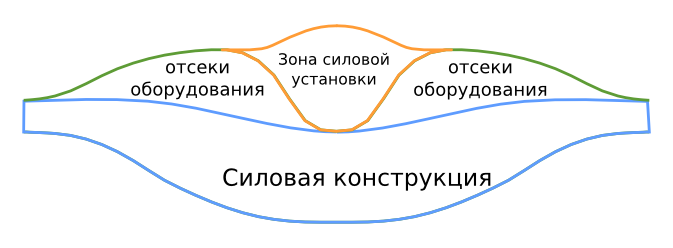
\includegraphics[width=0.8\textwidth]{OriginalSectionWithEngine}
\caption{Вид сечения центроплана в месте стыка передней кромки крыла и фюзеляжа с изображением двигателя}
\label{fig:OriginalSectionWithEngine}
\end{figure}


При такой конфигурации все хорошо (учтены требования малозаметности, аэродинамики).

Но это создает проблему обеспечения прочности центроплана, следовательно проблему весовой эффективности. Наше решение - критическое к созданию конструкции. Если не выйдет, всё летит к черту. Создаем модель по идеальной аэродинамике.

В настоящей работе рассматривается задача проектирования такой конструкции центроплана БПЛА с особенностью, с крылом большого удлинения.

В рамках решения задачи сформирован задел для дальнейшего решения многодисциплинарной задачи по выбору рациональной конфигурации с точки зрения критерия эффективности (по улучшению компоновки) с учетом возможного изменения внешней геометрии.

Описываем: для решения задачи в работе проведено концептуальное исследование зависимости весовых, прочностных и жесткостных характеристик конструкции от геометрических параметров, определяющих форму центроплана.

В работе также рассмотрены и приведены программные средства, предназначенные для решения подобных (параметрических, проектировочных) задач. И даны описания модификаций программы.

В работе сформирована КЭ параметрическая модель и проведены валидационные исследования этой модели. НА ней же проведены весовые оценки. 

 